% Options for packages loaded elsewhere
\PassOptionsToPackage{unicode}{hyperref}
\PassOptionsToPackage{hyphens}{url}
\PassOptionsToPackage{dvipsnames,svgnames,x11names}{xcolor}
%
\documentclass[
  letterpaper,
  DIV=11,
  numbers=noendperiod]{scrartcl}

\usepackage{amsmath,amssymb}
\usepackage{iftex}
\ifPDFTeX
  \usepackage[T1]{fontenc}
  \usepackage[utf8]{inputenc}
  \usepackage{textcomp} % provide euro and other symbols
\else % if luatex or xetex
  \usepackage{unicode-math}
  \defaultfontfeatures{Scale=MatchLowercase}
  \defaultfontfeatures[\rmfamily]{Ligatures=TeX,Scale=1}
\fi
\usepackage{lmodern}
\ifPDFTeX\else  
    % xetex/luatex font selection
\fi
% Use upquote if available, for straight quotes in verbatim environments
\IfFileExists{upquote.sty}{\usepackage{upquote}}{}
\IfFileExists{microtype.sty}{% use microtype if available
  \usepackage[]{microtype}
  \UseMicrotypeSet[protrusion]{basicmath} % disable protrusion for tt fonts
}{}
\makeatletter
\@ifundefined{KOMAClassName}{% if non-KOMA class
  \IfFileExists{parskip.sty}{%
    \usepackage{parskip}
  }{% else
    \setlength{\parindent}{0pt}
    \setlength{\parskip}{6pt plus 2pt minus 1pt}}
}{% if KOMA class
  \KOMAoptions{parskip=half}}
\makeatother
\usepackage{xcolor}
\setlength{\emergencystretch}{3em} % prevent overfull lines
\setcounter{secnumdepth}{-\maxdimen} % remove section numbering
% Make \paragraph and \subparagraph free-standing
\makeatletter
\ifx\paragraph\undefined\else
  \let\oldparagraph\paragraph
  \renewcommand{\paragraph}{
    \@ifstar
      \xxxParagraphStar
      \xxxParagraphNoStar
  }
  \newcommand{\xxxParagraphStar}[1]{\oldparagraph*{#1}\mbox{}}
  \newcommand{\xxxParagraphNoStar}[1]{\oldparagraph{#1}\mbox{}}
\fi
\ifx\subparagraph\undefined\else
  \let\oldsubparagraph\subparagraph
  \renewcommand{\subparagraph}{
    \@ifstar
      \xxxSubParagraphStar
      \xxxSubParagraphNoStar
  }
  \newcommand{\xxxSubParagraphStar}[1]{\oldsubparagraph*{#1}\mbox{}}
  \newcommand{\xxxSubParagraphNoStar}[1]{\oldsubparagraph{#1}\mbox{}}
\fi
\makeatother

\usepackage{color}
\usepackage{fancyvrb}
\newcommand{\VerbBar}{|}
\newcommand{\VERB}{\Verb[commandchars=\\\{\}]}
\DefineVerbatimEnvironment{Highlighting}{Verbatim}{commandchars=\\\{\}}
% Add ',fontsize=\small' for more characters per line
\usepackage{framed}
\definecolor{shadecolor}{RGB}{241,243,245}
\newenvironment{Shaded}{\begin{snugshade}}{\end{snugshade}}
\newcommand{\AlertTok}[1]{\textcolor[rgb]{0.68,0.00,0.00}{#1}}
\newcommand{\AnnotationTok}[1]{\textcolor[rgb]{0.37,0.37,0.37}{#1}}
\newcommand{\AttributeTok}[1]{\textcolor[rgb]{0.40,0.45,0.13}{#1}}
\newcommand{\BaseNTok}[1]{\textcolor[rgb]{0.68,0.00,0.00}{#1}}
\newcommand{\BuiltInTok}[1]{\textcolor[rgb]{0.00,0.23,0.31}{#1}}
\newcommand{\CharTok}[1]{\textcolor[rgb]{0.13,0.47,0.30}{#1}}
\newcommand{\CommentTok}[1]{\textcolor[rgb]{0.37,0.37,0.37}{#1}}
\newcommand{\CommentVarTok}[1]{\textcolor[rgb]{0.37,0.37,0.37}{\textit{#1}}}
\newcommand{\ConstantTok}[1]{\textcolor[rgb]{0.56,0.35,0.01}{#1}}
\newcommand{\ControlFlowTok}[1]{\textcolor[rgb]{0.00,0.23,0.31}{\textbf{#1}}}
\newcommand{\DataTypeTok}[1]{\textcolor[rgb]{0.68,0.00,0.00}{#1}}
\newcommand{\DecValTok}[1]{\textcolor[rgb]{0.68,0.00,0.00}{#1}}
\newcommand{\DocumentationTok}[1]{\textcolor[rgb]{0.37,0.37,0.37}{\textit{#1}}}
\newcommand{\ErrorTok}[1]{\textcolor[rgb]{0.68,0.00,0.00}{#1}}
\newcommand{\ExtensionTok}[1]{\textcolor[rgb]{0.00,0.23,0.31}{#1}}
\newcommand{\FloatTok}[1]{\textcolor[rgb]{0.68,0.00,0.00}{#1}}
\newcommand{\FunctionTok}[1]{\textcolor[rgb]{0.28,0.35,0.67}{#1}}
\newcommand{\ImportTok}[1]{\textcolor[rgb]{0.00,0.46,0.62}{#1}}
\newcommand{\InformationTok}[1]{\textcolor[rgb]{0.37,0.37,0.37}{#1}}
\newcommand{\KeywordTok}[1]{\textcolor[rgb]{0.00,0.23,0.31}{\textbf{#1}}}
\newcommand{\NormalTok}[1]{\textcolor[rgb]{0.00,0.23,0.31}{#1}}
\newcommand{\OperatorTok}[1]{\textcolor[rgb]{0.37,0.37,0.37}{#1}}
\newcommand{\OtherTok}[1]{\textcolor[rgb]{0.00,0.23,0.31}{#1}}
\newcommand{\PreprocessorTok}[1]{\textcolor[rgb]{0.68,0.00,0.00}{#1}}
\newcommand{\RegionMarkerTok}[1]{\textcolor[rgb]{0.00,0.23,0.31}{#1}}
\newcommand{\SpecialCharTok}[1]{\textcolor[rgb]{0.37,0.37,0.37}{#1}}
\newcommand{\SpecialStringTok}[1]{\textcolor[rgb]{0.13,0.47,0.30}{#1}}
\newcommand{\StringTok}[1]{\textcolor[rgb]{0.13,0.47,0.30}{#1}}
\newcommand{\VariableTok}[1]{\textcolor[rgb]{0.07,0.07,0.07}{#1}}
\newcommand{\VerbatimStringTok}[1]{\textcolor[rgb]{0.13,0.47,0.30}{#1}}
\newcommand{\WarningTok}[1]{\textcolor[rgb]{0.37,0.37,0.37}{\textit{#1}}}

\providecommand{\tightlist}{%
  \setlength{\itemsep}{0pt}\setlength{\parskip}{0pt}}\usepackage{longtable,booktabs,array}
\usepackage{calc} % for calculating minipage widths
% Correct order of tables after \paragraph or \subparagraph
\usepackage{etoolbox}
\makeatletter
\patchcmd\longtable{\par}{\if@noskipsec\mbox{}\fi\par}{}{}
\makeatother
% Allow footnotes in longtable head/foot
\IfFileExists{footnotehyper.sty}{\usepackage{footnotehyper}}{\usepackage{footnote}}
\makesavenoteenv{longtable}
\usepackage{graphicx}
\makeatletter
\def\maxwidth{\ifdim\Gin@nat@width>\linewidth\linewidth\else\Gin@nat@width\fi}
\def\maxheight{\ifdim\Gin@nat@height>\textheight\textheight\else\Gin@nat@height\fi}
\makeatother
% Scale images if necessary, so that they will not overflow the page
% margins by default, and it is still possible to overwrite the defaults
% using explicit options in \includegraphics[width, height, ...]{}
\setkeys{Gin}{width=\maxwidth,height=\maxheight,keepaspectratio}
% Set default figure placement to htbp
\makeatletter
\def\fps@figure{htbp}
\makeatother

\usepackage{fvextra}
\DefineVerbatimEnvironment{Highlighting}{Verbatim}{breaklines,commandchars=\\\{\}}
\KOMAoption{captions}{tableheading}
\makeatletter
\@ifpackageloaded{caption}{}{\usepackage{caption}}
\AtBeginDocument{%
\ifdefined\contentsname
  \renewcommand*\contentsname{Table of contents}
\else
  \newcommand\contentsname{Table of contents}
\fi
\ifdefined\listfigurename
  \renewcommand*\listfigurename{List of Figures}
\else
  \newcommand\listfigurename{List of Figures}
\fi
\ifdefined\listtablename
  \renewcommand*\listtablename{List of Tables}
\else
  \newcommand\listtablename{List of Tables}
\fi
\ifdefined\figurename
  \renewcommand*\figurename{Figure}
\else
  \newcommand\figurename{Figure}
\fi
\ifdefined\tablename
  \renewcommand*\tablename{Table}
\else
  \newcommand\tablename{Table}
\fi
}
\@ifpackageloaded{float}{}{\usepackage{float}}
\floatstyle{ruled}
\@ifundefined{c@chapter}{\newfloat{codelisting}{h}{lop}}{\newfloat{codelisting}{h}{lop}[chapter]}
\floatname{codelisting}{Listing}
\newcommand*\listoflistings{\listof{codelisting}{List of Listings}}
\makeatother
\makeatletter
\makeatother
\makeatletter
\@ifpackageloaded{caption}{}{\usepackage{caption}}
\@ifpackageloaded{subcaption}{}{\usepackage{subcaption}}
\makeatother

\ifLuaTeX
  \usepackage{selnolig}  % disable illegal ligatures
\fi
\usepackage{bookmark}

\IfFileExists{xurl.sty}{\usepackage{xurl}}{} % add URL line breaks if available
\urlstyle{same} % disable monospaced font for URLs
\hypersetup{
  pdftitle={Your Title},
  colorlinks=true,
  linkcolor={blue},
  filecolor={Maroon},
  citecolor={Blue},
  urlcolor={Blue},
  pdfcreator={LaTeX via pandoc}}


\title{Your Title}
\author{}
\date{}

\begin{document}
\maketitle

\RecustomVerbatimEnvironment{verbatim}{Verbatim}{
  showspaces = false,
  showtabs = false,
  breaksymbolleft={},
  breaklines
}


\textbf{PS4:} Due Sat Nov 2 at 5:00PM Central. Worth 100 points. We use
(\texttt{*}) to indicate a problem that we think might be time
consuming.

\subsection{Style Points (10 pts)}\label{style-points-10-pts}

Please refer to the minilesson on code style
\textbf{\href{https://uchicago.zoom.us/rec/share/pG_wQ-pHTQrJTmqNn4rcrw5V194M2H2s-2jdy8oVhWHkd_yZt9o162IWurpA-fxU.BIQlSgZLRYctvzp-}{here}}.

\subsection{Submission Steps (10 pts)}\label{submission-steps-10-pts}

\begin{enumerate}
\def\labelenumi{\arabic{enumi}.}
\tightlist
\item
  This problem set is a paired problem set.
\item
  Play paper, scissors, rock to determine who goes first. Call that
  person \emph{Partner 1}.

  \begin{itemize}
  \tightlist
  \item
    Partner 1 Lauren Laine, llaine:
  \item
    Partner 2 (Mohamed, cnet ID: shahim143 ):
  \end{itemize}
\item
  Partner 1 will accept the \texttt{ps4} and then share the link it
  creates with their partner. You can only share it with one partner so
  you will not be able to change it after your partner has accepted.
\item
  ``This submission is our work alone and complies with the 30538
  integrity policy.'' Add your initials to indicate your agreement:
  **\_\_** **\_\_**
\item
  ``I have uploaded the names of anyone else other than my partner and I
  worked with on the problem set
  \textbf{\href{https://docs.google.com/forms/d/185usrCREQaUbvAXpWhChkjghdGgmAZXA3lPWpXLLsts/edit}{here}}''
  (1 point)
\item
  Late coins used this pset: **\_\_** Late coins left after submission:
  **\_\_**
\item
  Knit your \texttt{ps4.qmd} to an PDF file to make \texttt{ps4.pdf},

  \begin{itemize}
  \tightlist
  \item
    The PDF should not be more than 25 pages. Use \texttt{head()} and
    re-size figures when appropriate.
  \end{itemize}
\item
  (Partner 1): push \texttt{ps4.qmd} and \texttt{ps4.pdf} to your github
  repo.
\item
  (Partner 1): submit \texttt{ps4.pdf} via Gradescope. Add your partner
  on Gradescope.
\item
  (Partner 1): tag your submission in Gradescope
\end{enumerate}

\textbf{Important:} Repositories are for tracking code. \textbf{Do not
commit the data or shapefiles to your repo.} The best way to do this is
with \texttt{.gitignore}, which we have covered in class. If you do
accidentally commit the data, Github has a
\href{https://docs.github.com/en/repositories/working-with-files/managing-large-files/about-large-files-on-github\#removing-files-from-a-repositorys-history}{guide}.
The best course of action depends on whether you have pushed yet. This
also means that both partners will have to download the initial raw data
and any data cleaning code will need to be re-run on both partners'
computers.

\subsection{Download and explore the Provider of Services (POS) file (10
pts)}\label{download-and-explore-the-provider-of-services-pos-file-10-pts}

\begin{enumerate}
\def\labelenumi{\arabic{enumi}.}
\item
  I pulled PRVDR\_CTGRY\_CD: provider category PRVDR\_CTGRY\_SBTYP\_CD:
  provider category subtype PRVDR\_NUM: CMS provider certification
  number PGM\_TRMNTN\_CD: termination Code FAC\_NAME: facility name
  ZIP\_CD: facility zip code
\item
  \begin{enumerate}
  \def\labelenumii{\alph{enumii}.}
  \tightlist
  \item
  \end{enumerate}
\end{enumerate}

\begin{Shaded}
\begin{Highlighting}[]
\CommentTok{\#import libraries}
\ImportTok{import}\NormalTok{ pandas }\ImportTok{as}\NormalTok{ pd}
\ImportTok{import}\NormalTok{ altair }\ImportTok{as}\NormalTok{ alt}
\ImportTok{import}\NormalTok{ shapely}
\ImportTok{from}\NormalTok{ shapely }\ImportTok{import}\NormalTok{ Polygon, Point}
\end{Highlighting}
\end{Shaded}

\begin{Shaded}
\begin{Highlighting}[]
\NormalTok{pos2016}\OperatorTok{=}\NormalTok{pd.read\_csv(}\VerbatimStringTok{r"C:\textbackslash{}Users\textbackslash{}laine\textbackslash{}OneDrive\textbackslash{}Documents\textbackslash{}GitHub\textbackslash{}problem{-}set{-}4{-}lauren{-}and{-}me\textbackslash{}pos2016.csv"}\NormalTok{)}
\end{Highlighting}
\end{Shaded}

\begin{Shaded}
\begin{Highlighting}[]
\NormalTok{short\_term\_hos\_2016}\OperatorTok{=}\NormalTok{pos2016[pos2016[}\StringTok{\textquotesingle{}PRVDR\_CTGRY\_CD\textquotesingle{}}\NormalTok{]}\OperatorTok{==}\DecValTok{1}\NormalTok{]}
\NormalTok{short\_term\_hos\_2016}\OperatorTok{=}\NormalTok{short\_term\_hos\_2016[short\_term\_hos\_2016[}\StringTok{\textquotesingle{}PRVDR\_CTGRY\_SBTYP\_CD\textquotesingle{}}\NormalTok{]}\OperatorTok{==}\DecValTok{1}\NormalTok{]}
\NormalTok{short\_term\_hos\_2016[}\StringTok{\textquotesingle{}year\textquotesingle{}}\NormalTok{]}\OperatorTok{=}\DecValTok{2016}
\BuiltInTok{print}\NormalTok{(}\BuiltInTok{len}\NormalTok{(short\_term\_hos\_2016))}
\end{Highlighting}
\end{Shaded}

\begin{verbatim}
7245
\end{verbatim}

There are 7245 hospitals reported in this data. This seems very low. b.
The Kaiser Family Foundation article reports that ``here are nearly
5,000 short-term, acute care hospitals in the United States''. That
estimate may be smaller because they are filtering down even further to
acute care hospitals.

Definitive Healthcare reports 3,873 short term acute care hospitals as
of April 2024. That estimate is much lower than the estimate from the
2016 data. There may have been many hospital closures since 2016 but it
seems unlikely that the number of short term hospitals would decrease by
almost 50\%.

Kaiser Family Foundation article:
https://www.kff.org/report-section/a-look-at-rural-hospital-closures-and-implications-for-access-to-care-three-case-studies-issue-brief/

Definitive Healthcare article:
https://www.definitivehc.com/blog/how-many-hospitals-are-in-the-us

\begin{enumerate}
\def\labelenumi{\arabic{enumi}.}
\setcounter{enumi}{2}
\tightlist
\item
\end{enumerate}

\begin{Shaded}
\begin{Highlighting}[]
\CommentTok{\# import and subset pos2017}
\NormalTok{pos2017}\OperatorTok{=}\NormalTok{pd.read\_csv(}\VerbatimStringTok{r"C:\textbackslash{}Users\textbackslash{}laine\textbackslash{}OneDrive\textbackslash{}Documents\textbackslash{}GitHub\textbackslash{}problem{-}set{-}4{-}lauren{-}and{-}me\textbackslash{}pos2017.csv"}\NormalTok{)}

\NormalTok{short\_term\_hos\_2017}\OperatorTok{=}\NormalTok{pos2017[pos2017[}\StringTok{\textquotesingle{}PRVDR\_CTGRY\_CD\textquotesingle{}}\NormalTok{]}\OperatorTok{==}\DecValTok{1}\NormalTok{]}
\NormalTok{short\_term\_hos\_2017}\OperatorTok{=}\NormalTok{short\_term\_hos\_2017[short\_term\_hos\_2017[}\StringTok{\textquotesingle{}PRVDR\_CTGRY\_SBTYP\_CD\textquotesingle{}}\NormalTok{]}\OperatorTok{==}\DecValTok{1}\NormalTok{]}
\NormalTok{short\_term\_hos\_2017[}\StringTok{\textquotesingle{}year\textquotesingle{}}\NormalTok{]}\OperatorTok{=}\DecValTok{2017}
\BuiltInTok{print}\NormalTok{(}\BuiltInTok{len}\NormalTok{(short\_term\_hos\_2017))}
\end{Highlighting}
\end{Shaded}

\begin{verbatim}
7260
\end{verbatim}

\begin{Shaded}
\begin{Highlighting}[]
\CommentTok{\# import and subset pos2018}
\NormalTok{pos2018}\OperatorTok{=}\NormalTok{pd.read\_csv(}\VerbatimStringTok{r"C:\textbackslash{}Users\textbackslash{}laine\textbackslash{}OneDrive\textbackslash{}Documents\textbackslash{}GitHub\textbackslash{}problem{-}set{-}4{-}lauren{-}and{-}me\textbackslash{}pos2018.csv"}\NormalTok{)}

\NormalTok{short\_term\_hos\_2018}\OperatorTok{=}\NormalTok{pos2018[pos2018[}\StringTok{\textquotesingle{}PRVDR\_CTGRY\_CD\textquotesingle{}}\NormalTok{]}\OperatorTok{==}\DecValTok{1}\NormalTok{]}
\NormalTok{short\_term\_hos\_2018}\OperatorTok{=}\NormalTok{short\_term\_hos\_2018[short\_term\_hos\_2018[}\StringTok{\textquotesingle{}PRVDR\_CTGRY\_SBTYP\_CD\textquotesingle{}}\NormalTok{]}\OperatorTok{==}\DecValTok{1}\NormalTok{]}
\NormalTok{short\_term\_hos\_2018[}\StringTok{\textquotesingle{}year\textquotesingle{}}\NormalTok{]}\OperatorTok{=}\DecValTok{2018}
\BuiltInTok{print}\NormalTok{(}\BuiltInTok{len}\NormalTok{(short\_term\_hos\_2018))}
\end{Highlighting}
\end{Shaded}

\begin{verbatim}
7277
\end{verbatim}

\begin{Shaded}
\begin{Highlighting}[]
\CommentTok{\# import and subset pos2019}
\NormalTok{pos2019}\OperatorTok{=}\NormalTok{pd.read\_csv(}\VerbatimStringTok{r"C:\textbackslash{}Users\textbackslash{}laine\textbackslash{}OneDrive\textbackslash{}Documents\textbackslash{}GitHub\textbackslash{}problem{-}set{-}4{-}lauren{-}and{-}me\textbackslash{}pos2019.csv"}\NormalTok{)}

\NormalTok{short\_term\_hos\_2019}\OperatorTok{=}\NormalTok{pos2019[pos2019[}\StringTok{\textquotesingle{}PRVDR\_CTGRY\_CD\textquotesingle{}}\NormalTok{]}\OperatorTok{==}\DecValTok{1}\NormalTok{]}
\NormalTok{short\_term\_hos\_2019}\OperatorTok{=}\NormalTok{short\_term\_hos\_2019[short\_term\_hos\_2019[}\StringTok{\textquotesingle{}PRVDR\_CTGRY\_SBTYP\_CD\textquotesingle{}}\NormalTok{]}\OperatorTok{==}\DecValTok{1}\NormalTok{]}
\NormalTok{short\_term\_hos\_2019[}\StringTok{\textquotesingle{}year\textquotesingle{}}\NormalTok{]}\OperatorTok{=}\DecValTok{2019}
\BuiltInTok{print}\NormalTok{(}\BuiltInTok{len}\NormalTok{(short\_term\_hos\_2019))}
\end{Highlighting}
\end{Shaded}

\begin{verbatim}
7303
\end{verbatim}

There are 7260 short term hospitals in the 2017 dataset. There are 7277
short term hospitals in the 2018 dataset. There are 7303 short term
hospitals in the 2019 dataset.

\begin{Shaded}
\begin{Highlighting}[]
\NormalTok{full\_df}\OperatorTok{=}\NormalTok{pd.concat([short\_term\_hos\_2016,short\_term\_hos\_2017,short\_term\_hos\_2018,short\_term\_hos\_2019])}
\end{Highlighting}
\end{Shaded}

\begin{Shaded}
\begin{Highlighting}[]
\NormalTok{alt.data\_transformers.disable\_max\_rows()}
\NormalTok{plot\_1\_3}\OperatorTok{=}\NormalTok{alt.Chart(full\_df, title}\OperatorTok{=}\StringTok{"Number of Short Term Hospitals by Year"}\NormalTok{).mark\_bar().encode(}
\NormalTok{    alt.X(}\StringTok{\textquotesingle{}year:O\textquotesingle{}}\NormalTok{),}
\NormalTok{    alt.Y(}\StringTok{\textquotesingle{}count(FAC\_NAME):Q\textquotesingle{}}\NormalTok{)}
\NormalTok{)}
\NormalTok{plot\_1\_3}
\end{Highlighting}
\end{Shaded}

\begin{verbatim}
alt.Chart(...)
\end{verbatim}

\begin{enumerate}
\def\labelenumi{\arabic{enumi}.}
\setcounter{enumi}{3}
\tightlist
\item
  \begin{enumerate}
  \def\labelenumii{\alph{enumii}.}
  \tightlist
  \item
  \end{enumerate}
\end{enumerate}

\begin{Shaded}
\begin{Highlighting}[]
\CommentTok{\#learned about the drop\_duplicates function }
\CommentTok{\#https://pandas.pydata.org/docs/reference/api/pandas.DataFrame.drop\_duplicates.html}
\NormalTok{unique\_nums2016}\OperatorTok{=}\NormalTok{short\_term\_hos\_2016.drop\_duplicates(subset}\OperatorTok{=}\StringTok{\textquotesingle{}PRVDR\_NUM\textquotesingle{}}\NormalTok{, keep}\OperatorTok{=}\StringTok{\textquotesingle{}first\textquotesingle{}}\NormalTok{)}
\CommentTok{\# check if duplicates were dropped}
\NormalTok{unique\_nums2016.groupby(}\StringTok{\textquotesingle{}PRVDR\_NUM\textquotesingle{}}\NormalTok{).size().head(}\DecValTok{15}\NormalTok{)}
\NormalTok{unique\_nums2017}\OperatorTok{=}\NormalTok{full\_df[full\_df[}\StringTok{\textquotesingle{}year\textquotesingle{}}\NormalTok{]}\OperatorTok{==}\DecValTok{2017}\NormalTok{].drop\_duplicates(subset}\OperatorTok{=}\StringTok{\textquotesingle{}PRVDR\_NUM\textquotesingle{}}\NormalTok{, keep}\OperatorTok{=}\StringTok{\textquotesingle{}first\textquotesingle{}}\NormalTok{)}
\NormalTok{unique\_nums2018}\OperatorTok{=}\NormalTok{full\_df[full\_df[}\StringTok{\textquotesingle{}year\textquotesingle{}}\NormalTok{]}\OperatorTok{==}\DecValTok{2018}\NormalTok{].drop\_duplicates(subset}\OperatorTok{=}\StringTok{\textquotesingle{}PRVDR\_NUM\textquotesingle{}}\NormalTok{, keep}\OperatorTok{=}\StringTok{\textquotesingle{}first\textquotesingle{}}\NormalTok{)}
\NormalTok{unique\_nums2019}\OperatorTok{=}\NormalTok{full\_df[full\_df[}\StringTok{\textquotesingle{}year\textquotesingle{}}\NormalTok{]}\OperatorTok{==}\DecValTok{2019}\NormalTok{].drop\_duplicates(subset}\OperatorTok{=}\StringTok{\textquotesingle{}PRVDR\_NUM\textquotesingle{}}\NormalTok{, keep}\OperatorTok{=}\StringTok{\textquotesingle{}first\textquotesingle{}}\NormalTok{)}
\NormalTok{full\_unique\_nums}\OperatorTok{=}\NormalTok{pd.concat([unique\_nums2016, unique\_nums2017, unique\_nums2018, unique\_nums2019])}
\end{Highlighting}
\end{Shaded}

\begin{Shaded}
\begin{Highlighting}[]
\NormalTok{unique\_hos\_plot}\OperatorTok{=}\NormalTok{alt.Chart(full\_unique\_nums).mark\_bar().encode(}
\NormalTok{    alt.X(}\StringTok{\textquotesingle{}year:O\textquotesingle{}}\NormalTok{).title(}\StringTok{"Year"}\NormalTok{),}
\NormalTok{    alt.Y(}\StringTok{\textquotesingle{}count(FAC\_NAME):Q\textquotesingle{}}\NormalTok{).title(}\StringTok{"Number of Observations"}\NormalTok{)}
\NormalTok{)}
\NormalTok{unique\_hos\_plot}
\end{Highlighting}
\end{Shaded}

\begin{verbatim}
alt.Chart(...)
\end{verbatim}

\begin{verbatim}
b.
\end{verbatim}

The unique provider number plot looks almost identical to the plot
before filtering out duplicates. This suggests that almost all of the
hospitals already had a unique provider number.

\subsection{Identify hospital closures in POS file (15 pts)
(*)}\label{identify-hospital-closures-in-pos-file-15-pts}

\begin{enumerate}
\def\labelenumi{\arabic{enumi}.}
\tightlist
\item
\end{enumerate}

\begin{Shaded}
\begin{Highlighting}[]
\NormalTok{list\_active\_hospitals\_2016 }\OperatorTok{=}\NormalTok{ full\_df[}
\NormalTok{    (full\_df[}\StringTok{\textquotesingle{}PRVDR\_CTGRY\_CD\textquotesingle{}}\NormalTok{] }\OperatorTok{==} \DecValTok{1}\NormalTok{) }\OperatorTok{\&} 
\NormalTok{    (full\_df[}\StringTok{\textquotesingle{}PRVDR\_CTGRY\_SBTYP\_CD\textquotesingle{}}\NormalTok{] }\OperatorTok{==} \DecValTok{1}\NormalTok{) }\OperatorTok{\&} 
\NormalTok{    (full\_df[}\StringTok{\textquotesingle{}PGM\_TRMNTN\_CD\textquotesingle{}}\NormalTok{] }\OperatorTok{==} \DecValTok{0}\NormalTok{) }\OperatorTok{\&} 
\NormalTok{    (full\_df[}\StringTok{\textquotesingle{}year\textquotesingle{}}\NormalTok{] }\OperatorTok{==} \DecValTok{2016}\NormalTok{)}
\NormalTok{]}

\NormalTok{providers\_active\_2016 }\OperatorTok{=}\NormalTok{ list\_active\_hospitals\_2016[}\StringTok{\textquotesingle{}PRVDR\_NUM\textquotesingle{}}\NormalTok{].unique()}

\NormalTok{closure\_records }\OperatorTok{=}\NormalTok{ []}

\NormalTok{years\_to\_check }\OperatorTok{=}\NormalTok{ [}\DecValTok{2017}\NormalTok{, }\DecValTok{2018}\NormalTok{, }\DecValTok{2019}\NormalTok{]}

\ControlFlowTok{for}\NormalTok{ provider }\KeywordTok{in}\NormalTok{ providers\_active\_2016:}
\NormalTok{    is\_closed }\OperatorTok{=} \VariableTok{True}
\NormalTok{    year\_of\_close }\OperatorTok{=} \VariableTok{None}
    
    \ControlFlowTok{for}\NormalTok{ year }\KeywordTok{in}\NormalTok{ years\_to\_check:}
\NormalTok{        yearly\_data }\OperatorTok{=}\NormalTok{ full\_df[}
\NormalTok{            (full\_df[}\StringTok{\textquotesingle{}PRVDR\_NUM\textquotesingle{}}\NormalTok{] }\OperatorTok{==}\NormalTok{ provider) }\OperatorTok{\&} 
\NormalTok{            (full\_df[}\StringTok{\textquotesingle{}PRVDR\_CTGRY\_CD\textquotesingle{}}\NormalTok{] }\OperatorTok{==} \DecValTok{1}\NormalTok{) }\OperatorTok{\&} 
\NormalTok{            (full\_df[}\StringTok{\textquotesingle{}PRVDR\_CTGRY\_SBTYP\_CD\textquotesingle{}}\NormalTok{] }\OperatorTok{==} \DecValTok{1}\NormalTok{) }\OperatorTok{\&} 
\NormalTok{            (full\_df[}\StringTok{\textquotesingle{}year\textquotesingle{}}\NormalTok{] }\OperatorTok{==}\NormalTok{ year)}
\NormalTok{        ]}
        
        \ControlFlowTok{if} \KeywordTok{not}\NormalTok{ yearly\_data.empty }\KeywordTok{and}\NormalTok{ yearly\_data[}\StringTok{\textquotesingle{}PGM\_TRMNTN\_CD\textquotesingle{}}\NormalTok{].values[}\DecValTok{0}\NormalTok{] }\OperatorTok{==} \DecValTok{0}\NormalTok{:}
\NormalTok{            is\_closed }\OperatorTok{=} \VariableTok{False}
            \ControlFlowTok{break}
        \ControlFlowTok{elif} \KeywordTok{not}\NormalTok{ yearly\_data.empty:}
\NormalTok{            year\_of\_close }\OperatorTok{=}\NormalTok{ year}
    
    \ControlFlowTok{if}\NormalTok{ is\_closed:}
\NormalTok{        hospital\_info }\OperatorTok{=}\NormalTok{ list\_active\_hospitals\_2016[list\_active\_hospitals\_2016[}\StringTok{\textquotesingle{}PRVDR\_NUM\textquotesingle{}}\NormalTok{] }\OperatorTok{==}\NormalTok{ provider].iloc[}\DecValTok{0}\NormalTok{]}
\NormalTok{        closure\_records.append(\{}
            \StringTok{\textquotesingle{}FAC\_NAME\textquotesingle{}}\NormalTok{: hospital\_info[}\StringTok{\textquotesingle{}FAC\_NAME\textquotesingle{}}\NormalTok{],}
            \StringTok{\textquotesingle{}ZIP\_CD\textquotesingle{}}\NormalTok{: hospital\_info[}\StringTok{\textquotesingle{}ZIP\_CD\textquotesingle{}}\NormalTok{],}
            \StringTok{\textquotesingle{}closure\_year\textquotesingle{}}\NormalTok{: year\_of\_close}
\NormalTok{        \})}

\NormalTok{closures\_data }\OperatorTok{=}\NormalTok{ pd.DataFrame(closure\_records)}

\NormalTok{total\_closures\_by\_2019 }\OperatorTok{=}\NormalTok{ closures\_data.shape[}\DecValTok{0}\NormalTok{]}
\BuiltInTok{print}\NormalTok{(}\SpecialStringTok{f"Total suspected closures by 2019: }\SpecialCharTok{\{}\NormalTok{total\_closures\_by\_2019}\SpecialCharTok{\}}\SpecialStringTok{"}\NormalTok{)}
\end{Highlighting}
\end{Shaded}

\begin{verbatim}
Total suspected closures by 2019: 40
\end{verbatim}

'\,'\,' List of hospitals are there that fit this definition are 40
'\,'\,' 2.

\begin{Shaded}
\begin{Highlighting}[]
\NormalTok{sorted\_closures\_data }\OperatorTok{=}\NormalTok{ closures\_data.sort\_values(by}\OperatorTok{=}\StringTok{\textquotesingle{}FAC\_NAME\textquotesingle{}}\NormalTok{)[[}\StringTok{\textquotesingle{}FAC\_NAME\textquotesingle{}}\NormalTok{, }\StringTok{\textquotesingle{}closure\_year\textquotesingle{}}\NormalTok{]]}

\NormalTok{sorted\_closures\_data.head(}\DecValTok{10}\NormalTok{)}
\end{Highlighting}
\end{Shaded}

\begin{longtable}[]{@{}lll@{}}
\toprule\noalign{}
& FAC\_NAME & closure\_year \\
\midrule\noalign{}
\endhead
\bottomrule\noalign{}
\endlastfoot
0 & ABRAZO MARYVALE CAMPUS & 2017 \\
1 & ADVENTIST MEDICAL CENTER - CENTRAL VALLEY & 2017 \\
15 & ALBANY MEDICAL CENTER / SOUTH CLINICAL CAMPUS & 2019 \\
29 & ALLEGIANCE SPECIALTY HOSPITAL OF KILGORE & 2019 \\
3 & ARKANSAS VALLEY REGIONAL MEDICAL CENTER & 2017 \\
11 & BANNER CHURCHILL COMMUNITY HOSPITAL & 2019 \\
9 & BAYSTATE MARY LANE HOSPITAL & 2019 \\
16 & CAROLINAS CONTINUECARE HOSPITAL AT UNIVERSITY & 2019 \\
26 & CHILDREN\textquotesingle S HOSPITAL -SCOTT \& WHITE HEALTHCARE &
2019 \\
6 & CONTINUECARE HOSPITAL AT BAPTIST HEALTH PADUCAH & 2019 \\
\end{longtable}

\begin{enumerate}
\def\labelenumi{\arabic{enumi}.}
\setcounter{enumi}{2}
\tightlist
\item
  \begin{enumerate}
  \def\labelenumii{\alph{enumii}.}
  \tightlist
  \item
  \end{enumerate}
\end{enumerate}

\begin{Shaded}
\begin{Highlighting}[]
\NormalTok{active\_hospitals\_by\_zip\_year }\OperatorTok{=}\NormalTok{ full\_df[(full\_df[}\StringTok{\textquotesingle{}PGM\_TRMNTN\_CD\textquotesingle{}}\NormalTok{] }\OperatorTok{==} \DecValTok{0}\NormalTok{) }\OperatorTok{\&} 
\NormalTok{                                       (full\_df[}\StringTok{\textquotesingle{}PRVDR\_CTGRY\_CD\textquotesingle{}}\NormalTok{] }\OperatorTok{==} \DecValTok{1}\NormalTok{) }\OperatorTok{\&} 
\NormalTok{                                       (full\_df[}\StringTok{\textquotesingle{}PRVDR\_CTGRY\_SBTYP\_CD\textquotesingle{}}\NormalTok{] }\OperatorTok{==} \DecValTok{1}\NormalTok{)]}
\NormalTok{active\_ones }\OperatorTok{=}\NormalTok{ active\_hospitals\_by\_zip\_year.groupby([}\StringTok{\textquotesingle{}ZIP\_CD\textquotesingle{}}\NormalTok{, }\StringTok{\textquotesingle{}year\textquotesingle{}}\NormalTok{]).size().reset\_index(name}\OperatorTok{=}\StringTok{\textquotesingle{}active\_count\textquotesingle{}}\NormalTok{)}

\NormalTok{closures\_data }\OperatorTok{=}\NormalTok{ closures\_data.merge(active\_ones, left\_on}\OperatorTok{=}\NormalTok{[}\StringTok{\textquotesingle{}ZIP\_CD\textquotesingle{}}\NormalTok{, }\StringTok{\textquotesingle{}closure\_year\textquotesingle{}}\NormalTok{], right\_on}\OperatorTok{=}\NormalTok{[}\StringTok{\textquotesingle{}ZIP\_CD\textquotesingle{}}\NormalTok{, }\StringTok{\textquotesingle{}year\textquotesingle{}}\NormalTok{], how}\OperatorTok{=}\StringTok{\textquotesingle{}left\textquotesingle{}}\NormalTok{)}
\NormalTok{closures\_data }\OperatorTok{=}\NormalTok{ closures\_data.rename(columns}\OperatorTok{=}\NormalTok{\{}\StringTok{\textquotesingle{}active\_count\textquotesingle{}}\NormalTok{: }\StringTok{\textquotesingle{}closure\_year\_active\_count\textquotesingle{}}\NormalTok{\})}

\NormalTok{closures\_data }\OperatorTok{=}\NormalTok{ closures\_data.merge(}
\NormalTok{    active\_ones,}
\NormalTok{    left\_on}\OperatorTok{=}\NormalTok{[}\StringTok{\textquotesingle{}ZIP\_CD\textquotesingle{}}\NormalTok{, }\StringTok{\textquotesingle{}closure\_year\textquotesingle{}}\NormalTok{],}
\NormalTok{    right\_on}\OperatorTok{=}\NormalTok{[}\StringTok{\textquotesingle{}ZIP\_CD\textquotesingle{}}\NormalTok{, }\StringTok{\textquotesingle{}year\textquotesingle{}}\NormalTok{],}
\NormalTok{    suffixes}\OperatorTok{=}\NormalTok{(}\StringTok{\textquotesingle{}\textquotesingle{}}\NormalTok{, }\StringTok{\textquotesingle{}\_next\textquotesingle{}}\NormalTok{),}
\NormalTok{    how}\OperatorTok{=}\StringTok{\textquotesingle{}left\textquotesingle{}}
\NormalTok{)}
\NormalTok{closures\_data }\OperatorTok{=}\NormalTok{ closures\_data.rename(columns}\OperatorTok{=}\NormalTok{\{}\StringTok{\textquotesingle{}active\_count\textquotesingle{}}\NormalTok{: }\StringTok{\textquotesingle{}next\_year\_active\_count\textquotesingle{}}\NormalTok{\})}

\NormalTok{closures\_data[}\StringTok{\textquotesingle{}potential\_acquisition\_merger\textquotesingle{}}\NormalTok{] }\OperatorTok{=}\NormalTok{ closures\_data[}\StringTok{\textquotesingle{}next\_year\_active\_count\textquotesingle{}}\NormalTok{] }\OperatorTok{\textgreater{}=}\NormalTok{ closures\_data[}\StringTok{\textquotesingle{}closure\_year\_active\_count\textquotesingle{}}\NormalTok{]}

\NormalTok{potential\_acquisition\_mergers }\OperatorTok{=}\NormalTok{ closures\_data[closures\_data[}\StringTok{\textquotesingle{}potential\_acquisition\_merger\textquotesingle{}}\NormalTok{]].copy()}
\NormalTok{potential\_acquisition\_merger\_count }\OperatorTok{=}\NormalTok{ potential\_acquisition\_mergers.shape[}\DecValTok{0}\NormalTok{]}

\BuiltInTok{print}\NormalTok{(}\SpecialStringTok{f"Number of hospitals potentially closed due to mergers/acquisitions: }\SpecialCharTok{\{}\NormalTok{potential\_acquisition\_merger\_count}\SpecialCharTok{\}}\SpecialStringTok{"}\NormalTok{)}
\end{Highlighting}
\end{Shaded}

\begin{verbatim}
Number of hospitals potentially closed due to mergers/acquisitions: 13
\end{verbatim}

\begin{verbatim}
b.
\end{verbatim}

\begin{Shaded}
\begin{Highlighting}[]
\NormalTok{corrected\_closures\_data }\OperatorTok{=}\NormalTok{ closures\_data[}\OperatorTok{\textasciitilde{}}\NormalTok{closures\_data[}\StringTok{\textquotesingle{}potential\_acquisition\_merger\textquotesingle{}}\NormalTok{]]}

\NormalTok{remaining\_closures\_count }\OperatorTok{=}\NormalTok{ corrected\_closures\_data.shape[}\DecValTok{0}\NormalTok{]}
\BuiltInTok{print}\NormalTok{(}\SpecialStringTok{f"Number of suspected closures after correcting for mergers/acquisitions: }\SpecialCharTok{\{}\NormalTok{remaining\_closures\_count}\SpecialCharTok{\}}\SpecialStringTok{"}\NormalTok{)}
\end{Highlighting}
\end{Shaded}

\begin{verbatim}
Number of suspected closures after correcting for mergers/acquisitions: 27
\end{verbatim}

\begin{verbatim}
c.
\end{verbatim}

\begin{Shaded}
\begin{Highlighting}[]
\NormalTok{sorted\_corrected\_closures }\OperatorTok{=}\NormalTok{ corrected\_closures\_data.sort\_values(by}\OperatorTok{=}\StringTok{\textquotesingle{}FAC\_NAME\textquotesingle{}}\NormalTok{)[[}\StringTok{\textquotesingle{}FAC\_NAME\textquotesingle{}}\NormalTok{, }\StringTok{\textquotesingle{}ZIP\_CD\textquotesingle{}}\NormalTok{, }\StringTok{\textquotesingle{}closure\_year\textquotesingle{}}\NormalTok{]]}

\NormalTok{sorted\_corrected\_closures.head(}\DecValTok{10}\NormalTok{)}
\end{Highlighting}
\end{Shaded}

\begin{longtable}[]{@{}llll@{}}
\toprule\noalign{}
& FAC\_NAME & ZIP\_CD & closure\_year \\
\midrule\noalign{}
\endhead
\bottomrule\noalign{}
\endlastfoot
0 & ABRAZO MARYVALE CAMPUS & 85031.0 & 2017 \\
29 & ALLEGIANCE SPECIALTY HOSPITAL OF KILGORE & 75662.0 & 2019 \\
3 & ARKANSAS VALLEY REGIONAL MEDICAL CENTER & 81050.0 & 2017 \\
11 & BANNER CHURCHILL COMMUNITY HOSPITAL & 89406.0 & 2019 \\
9 & BAYSTATE MARY LANE HOSPITAL & 1082.0 & 2019 \\
16 & CAROLINAS CONTINUECARE HOSPITAL AT UNIVERSITY & 28217.0 & 2019 \\
26 & CHILDREN\textquotesingle S HOSPITAL -SCOTT \& WHITE HEALTHCARE &
76502.0 & 2019 \\
31 & DIMMIT REGIONAL HOSPITAL & 78834.0 & 2019 \\
32 & EAST TEXAS MEDICAL CENTER TRINITY & 75862.0 & 2019 \\
2 & FALLBROOK HOSPITAL DISTRICT & 92028.0 & 2017 \\
\end{longtable}

\subsection{Download Census zip code shapefile (10
pt)}\label{download-census-zip-code-shapefile-10-pt}

\begin{enumerate}
\def\labelenumi{\arabic{enumi}.}
\item
  \begin{enumerate}
  \def\labelenumii{\alph{enumii}.}
  \item
    The file types are .dbf, .prj, .shp, .shx, and .xml. The .dbf file
    has attribute information The .prj file describes the Coordinate
    Reference System. The .shp has feature geometrics. The .shx has a
    positional index. The .xml file has details on where the data was
    obtained, and how often it is updated, and other notes on data use.
  \item
    The .dbf file is 6,275 KB The .prj file is 1 KB The .shp file is
    817,915 KB The .shx file is 259 KB The .xml file is 16 KB
  \end{enumerate}
\item
\end{enumerate}

\begin{Shaded}
\begin{Highlighting}[]
\ImportTok{import}\NormalTok{ geopandas }\ImportTok{as}\NormalTok{ gpd}
\NormalTok{census\_data}\OperatorTok{=}\NormalTok{gpd.read\_file(}\VerbatimStringTok{r"C:\textbackslash{}Users\textbackslash{}laine\textbackslash{}OneDrive\textbackslash{}Documents\textbackslash{}GitHub\textbackslash{}problem{-}set{-}4{-}lauren{-}and{-}me\textbackslash{}gz\_2010\_us\_860\_00\_500k.shp"}\NormalTok{)}
\end{Highlighting}
\end{Shaded}

\begin{Shaded}
\begin{Highlighting}[]
\NormalTok{census\_data.head()}
\CommentTok{\# used ChatGPT to Debug and filter to multipel prefixes. }
\CommentTok{\#prompt "How can I filter to multiple startswith strings"}
\NormalTok{prefixes}\OperatorTok{=}\NormalTok{(}\StringTok{\textquotesingle{}75\textquotesingle{}}\NormalTok{, }\StringTok{\textquotesingle{}76\textquotesingle{}}\NormalTok{, }\StringTok{\textquotesingle{}77\textquotesingle{}}\NormalTok{, }\StringTok{\textquotesingle{}78\textquotesingle{}}\NormalTok{, }\StringTok{\textquotesingle{}79\textquotesingle{}}\NormalTok{)}
\NormalTok{census\_data[}\StringTok{\textquotesingle{}texas\textquotesingle{}}\NormalTok{]}\OperatorTok{=}\NormalTok{census\_data[}\StringTok{\textquotesingle{}ZCTA5\textquotesingle{}}\NormalTok{].}\BuiltInTok{map}\NormalTok{(}\KeywordTok{lambda}\NormalTok{ x: }\DecValTok{1} \ControlFlowTok{if} \BuiltInTok{any}\NormalTok{(}\BuiltInTok{str}\NormalTok{(x).startswith(prefix) }\ControlFlowTok{for}\NormalTok{ prefix }\KeywordTok{in}\NormalTok{ prefixes)}\ControlFlowTok{else} \DecValTok{0}\NormalTok{)}
\NormalTok{texas\_data}\OperatorTok{=}\NormalTok{census\_data[census\_data[}\StringTok{\textquotesingle{}texas\textquotesingle{}}\NormalTok{]}\OperatorTok{==}\DecValTok{1}\NormalTok{]}
\end{Highlighting}
\end{Shaded}

\begin{Shaded}
\begin{Highlighting}[]
\NormalTok{geometry}\OperatorTok{=}\NormalTok{texas\_data[[}\StringTok{\textquotesingle{}ZCTA5\textquotesingle{}}\NormalTok{, }\StringTok{\textquotesingle{}geometry\textquotesingle{}}\NormalTok{]]}
\NormalTok{geometry.dtypes}
\NormalTok{geometry}\OperatorTok{=}\NormalTok{geometry.dropna()}
\NormalTok{geometry[}\StringTok{\textquotesingle{}ZCTA5\textquotesingle{}}\NormalTok{]}\OperatorTok{=}\NormalTok{pd.to\_numeric(geometry[}\StringTok{\textquotesingle{}ZCTA5\textquotesingle{}}\NormalTok{])}
\NormalTok{geometry.dtypes}
\end{Highlighting}
\end{Shaded}

\begin{verbatim}
ZCTA5          int64
geometry    geometry
dtype: object
\end{verbatim}

\#check geometry

\begin{Shaded}
\begin{Highlighting}[]
\ImportTok{import}\NormalTok{ matplotlib.pyplot }\ImportTok{as}\NormalTok{ plt}
\NormalTok{geometry.plot(facecolor}\OperatorTok{=}\StringTok{\textquotesingle{}none\textquotesingle{}}\NormalTok{).set\_axis\_off()}
\end{Highlighting}
\end{Shaded}

\includegraphics{pset4_template_files/figure-pdf/cell-20-output-1.pdf}

\begin{Shaded}
\begin{Highlighting}[]
\NormalTok{counts}\OperatorTok{=}\NormalTok{short\_term\_hos\_2016[}\StringTok{\textquotesingle{}ZIP\_CD\textquotesingle{}}\NormalTok{].value\_counts()}
\NormalTok{counts}\OperatorTok{=}\NormalTok{counts.reset\_index()}
\NormalTok{counts[}\StringTok{\textquotesingle{}ZIP\_CD\textquotesingle{}}\NormalTok{]}\OperatorTok{=}\NormalTok{counts[}\StringTok{\textquotesingle{}ZIP\_CD\textquotesingle{}}\NormalTok{].}\BuiltInTok{map}\NormalTok{(}\BuiltInTok{int}\NormalTok{)}
\NormalTok{counts.dtypes}
\end{Highlighting}
\end{Shaded}

\begin{verbatim}
ZIP_CD    int64
count     int64
dtype: object
\end{verbatim}

\begin{Shaded}
\begin{Highlighting}[]
\CommentTok{\#merge}
\NormalTok{merge}\OperatorTok{=}\NormalTok{geometry.merge(counts, left\_on}\OperatorTok{=}\StringTok{\textquotesingle{}ZCTA5\textquotesingle{}}\NormalTok{, right\_on}\OperatorTok{=}\StringTok{\textquotesingle{}ZIP\_CD\textquotesingle{}}\NormalTok{, how}\OperatorTok{=}\StringTok{\textquotesingle{}left\textquotesingle{}}\NormalTok{)}
\NormalTok{merge}\OperatorTok{=}\NormalTok{merge.fillna(}\DecValTok{0}\NormalTok{)}
\NormalTok{merge}\OperatorTok{=}\NormalTok{gpd.GeoDataFrame(merge, geometry}\OperatorTok{=}\StringTok{\textquotesingle{}geometry\textquotesingle{}}\NormalTok{)}
\end{Highlighting}
\end{Shaded}

\begin{Shaded}
\begin{Highlighting}[]
\CommentTok{\#plot}
\NormalTok{plot}\OperatorTok{=}\NormalTok{merge.plot()}
\end{Highlighting}
\end{Shaded}

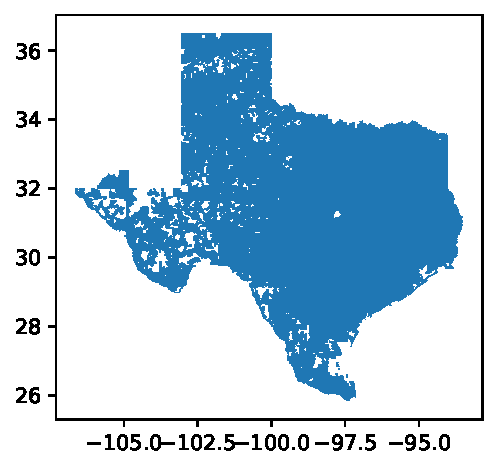
\includegraphics{pset4_template_files/figure-pdf/cell-23-output-1.pdf}

\begin{Shaded}
\begin{Highlighting}[]
\NormalTok{plot}\OperatorTok{=}\NormalTok{merge.plot(column}\OperatorTok{=}\StringTok{\textquotesingle{}count\textquotesingle{}}\NormalTok{, legend}\OperatorTok{=}\VariableTok{True}\NormalTok{).set\_axis\_off()}
\end{Highlighting}
\end{Shaded}

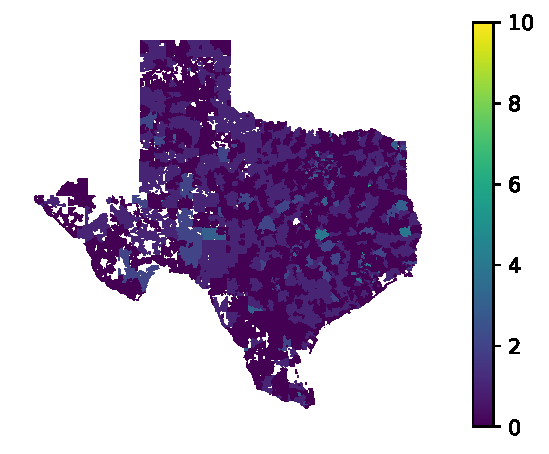
\includegraphics{pset4_template_files/figure-pdf/cell-24-output-1.pdf}

\subsection{Calculate zip code's distance to the nearest hospital (20
pts)
(*)}\label{calculate-zip-codes-distance-to-the-nearest-hospital-20-pts}

\begin{enumerate}
\def\labelenumi{\arabic{enumi}.}
\tightlist
\item
\end{enumerate}

\begin{Shaded}
\begin{Highlighting}[]
\NormalTok{census\_data}
\NormalTok{zips\_all\_centroids}\OperatorTok{=}\NormalTok{census\_data}
\NormalTok{zips\_all\_centroids[}\StringTok{\textquotesingle{}centroid\textquotesingle{}}\NormalTok{]}\OperatorTok{=}\NormalTok{zips\_all\_centroids.centroid}
\NormalTok{zips\_all\_centroids.shape}
\NormalTok{zips\_all\_centroids.head()}
\end{Highlighting}
\end{Shaded}

\begin{verbatim}
C:\Users\laine\AppData\Local\Temp\ipykernel_1060\2924888404.py:3: UserWarning: Geometry is in a geographic CRS. Results from 'centroid' are likely incorrect. Use 'GeoSeries.to_crs()' to re-project geometries to a projected CRS before this operation.

  zips_all_centroids['centroid']=zips_all_centroids.centroid
\end{verbatim}

\begin{longtable}[]{@{}lllllllll@{}}
\toprule\noalign{}
& GEO\_ID & ZCTA5 & NAME & LSAD & CENSUSAREA & geometry & texas &
centroid \\
\midrule\noalign{}
\endhead
\bottomrule\noalign{}
\endlastfoot
0 & 8600000US01040 & 01040 & 01040 & ZCTA5 & 21.281 & POLYGON
((-72.62734 42.16203, -72.62764 42.162... & 0 & POINT (-72.64107
42.21257) \\
1 & 8600000US01050 & 01050 & 01050 & ZCTA5 & 38.329 & POLYGON
((-72.95393 42.34379, -72.95385 42.343... & 0 & POINT (-72.86985
42.28786) \\
2 & 8600000US01053 & 01053 & 01053 & ZCTA5 & 5.131 & POLYGON ((-72.68286
42.37002, -72.68287 42.369... & 0 & POINT (-72.71162 42.35349) \\
3 & 8600000US01056 & 01056 & 01056 & ZCTA5 & 27.205 & POLYGON
((-72.39529 42.18476, -72.39653 42.183... & 0 & POINT (-72.45805
42.19215) \\
4 & 8600000US01057 & 01057 & 01057 & ZCTA5 & 44.907 & MULTIPOLYGON
(((-72.39191 42.08066, -72.39077 ... & 0 & POINT (-72.3243 42.09165) \\
\end{longtable}

The resulting dataframe as 33,120 rows and 8 columns.

The columns are GEO\_ID: Geographic Identifier- Fully Concatenated
Geographic Code ZCTA5: Five digit zipcode NAME: Base Name with
Translated Legal/Statistical Area Description (the same as ZCTA5) LSAD:
Legal Statistical Area Description CENSUSAREA: geometry: the polygon or
multipolygon for each zipcode texax: The indicator variable I created
that shows 1 if the zipcode is in texas and 0 otherwise centroid: the
centroid of the zipcode Source for column definitions:
https://tigerweb.geo.census.gov/tigerwebmain/TIGERweb\_attribute\_glossary.html

\begin{enumerate}
\def\labelenumi{\arabic{enumi}.}
\setcounter{enumi}{1}
\tightlist
\item
\end{enumerate}

\begin{Shaded}
\begin{Highlighting}[]
\NormalTok{zips\_texas\_centroids}\OperatorTok{=}\NormalTok{zips\_all\_centroids[zips\_all\_centroids[}\StringTok{\textquotesingle{}texas\textquotesingle{}}\NormalTok{]}\OperatorTok{==}\DecValTok{1}\NormalTok{]}
\end{Highlighting}
\end{Shaded}

Bordering States NM: 870-884 OK:73-34 AK:716-729 LA: 700-715

\begin{Shaded}
\begin{Highlighting}[]
\NormalTok{border\_prefixes}\OperatorTok{=}\NormalTok{(}\StringTok{\textquotesingle{}870\textquotesingle{}}\NormalTok{, }\StringTok{\textquotesingle{}871\textquotesingle{}}\NormalTok{, }\StringTok{\textquotesingle{}872\textquotesingle{}}\NormalTok{, }\StringTok{\textquotesingle{}873\textquotesingle{}}\NormalTok{, }\StringTok{\textquotesingle{}874\textquotesingle{}}\NormalTok{, }\StringTok{\textquotesingle{}875\textquotesingle{}}\NormalTok{, }\StringTok{\textquotesingle{}876\textquotesingle{}}\NormalTok{, }\StringTok{\textquotesingle{}877\textquotesingle{}}\NormalTok{, }\StringTok{\textquotesingle{}878\textquotesingle{}}\NormalTok{, }\StringTok{\textquotesingle{}879\textquotesingle{}}\NormalTok{, }\StringTok{\textquotesingle{}880\textquotesingle{}}\NormalTok{, }\StringTok{\textquotesingle{}881\textquotesingle{}}\NormalTok{, }\StringTok{\textquotesingle{}882\textquotesingle{}}\NormalTok{, }\StringTok{\textquotesingle{}883\textquotesingle{}}\NormalTok{, }\StringTok{\textquotesingle{}884\textquotesingle{}}\NormalTok{, }\StringTok{\textquotesingle{}73\textquotesingle{}}\NormalTok{, }\StringTok{\textquotesingle{}74\textquotesingle{}}\NormalTok{, }\StringTok{\textquotesingle{}716\textquotesingle{}}\NormalTok{, }\StringTok{\textquotesingle{}717\textquotesingle{}}\NormalTok{, }\StringTok{\textquotesingle{}718\textquotesingle{}}\NormalTok{, }\StringTok{\textquotesingle{}719\textquotesingle{}}\NormalTok{, }\StringTok{\textquotesingle{}720\textquotesingle{}}\NormalTok{, }\StringTok{\textquotesingle{}721\textquotesingle{}}\NormalTok{, }\StringTok{\textquotesingle{}722\textquotesingle{}}\NormalTok{, }\StringTok{\textquotesingle{}723\textquotesingle{}}\NormalTok{,}\StringTok{\textquotesingle{}724\textquotesingle{}}\NormalTok{,}\StringTok{\textquotesingle{}725\textquotesingle{}}\NormalTok{,}\StringTok{\textquotesingle{}726\textquotesingle{}}\NormalTok{,}\StringTok{\textquotesingle{}728\textquotesingle{}}\NormalTok{,}\StringTok{\textquotesingle{}729\textquotesingle{}}\NormalTok{, }\StringTok{\textquotesingle{}700\textquotesingle{}}\NormalTok{, }\StringTok{\textquotesingle{}701\textquotesingle{}}\NormalTok{,}\StringTok{\textquotesingle{}702\textquotesingle{}}\NormalTok{,}\StringTok{\textquotesingle{}703\textquotesingle{}}\NormalTok{,}\StringTok{\textquotesingle{}704\textquotesingle{}}\NormalTok{,}\StringTok{\textquotesingle{}705\textquotesingle{}}\NormalTok{,}\StringTok{\textquotesingle{}706\textquotesingle{}}\NormalTok{,}\StringTok{\textquotesingle{}707\textquotesingle{}}\NormalTok{,}\StringTok{\textquotesingle{}708\textquotesingle{}}\NormalTok{,}\StringTok{\textquotesingle{}709\textquotesingle{}}\NormalTok{,}\StringTok{\textquotesingle{}710\textquotesingle{}}\NormalTok{,}\StringTok{\textquotesingle{}711\textquotesingle{}}\NormalTok{,}\StringTok{\textquotesingle{}712\textquotesingle{}}\NormalTok{,}\StringTok{\textquotesingle{}713\textquotesingle{}}\NormalTok{,}\StringTok{\textquotesingle{}714\textquotesingle{}}\NormalTok{,}\StringTok{\textquotesingle{}715\textquotesingle{}}\NormalTok{)}
\NormalTok{border\_prefixes}\OperatorTok{=}\NormalTok{border\_prefixes}\OperatorTok{+}\NormalTok{prefixes}
\NormalTok{zips\_all\_centroids[}\StringTok{\textquotesingle{}border\textquotesingle{}}\NormalTok{]}\OperatorTok{=}\NormalTok{zips\_all\_centroids[}\StringTok{\textquotesingle{}ZCTA5\textquotesingle{}}\NormalTok{].}\BuiltInTok{map}\NormalTok{(}\KeywordTok{lambda}\NormalTok{ x:}\DecValTok{1} \ControlFlowTok{if} \BuiltInTok{any}\NormalTok{(}\BuiltInTok{str}\NormalTok{(x).startswith(prefix)}\ControlFlowTok{for}\NormalTok{ prefix }\KeywordTok{in}\NormalTok{ border\_prefixes)}\ControlFlowTok{else} \DecValTok{0}\NormalTok{)}
\NormalTok{zips\_texas\_borderstates\_centroids}\OperatorTok{=}\NormalTok{zips\_all\_centroids[zips\_all\_centroids[}\StringTok{\textquotesingle{}border\textquotesingle{}}\NormalTok{]}\OperatorTok{==}\DecValTok{1}\NormalTok{]}
\end{Highlighting}
\end{Shaded}

\begin{Shaded}
\begin{Highlighting}[]
\NormalTok{unique\_nums2016}\OperatorTok{=}\NormalTok{short\_term\_hos\_2016.drop\_duplicates(subset}\OperatorTok{=}\StringTok{\textquotesingle{}PRVDR\_NUM\textquotesingle{}}\NormalTok{, keep}\OperatorTok{=}\StringTok{\textquotesingle{}first\textquotesingle{}}\NormalTok{)}
\end{Highlighting}
\end{Shaded}

\begin{Shaded}
\begin{Highlighting}[]
\NormalTok{unique\_zips\_texas\_centroids}\OperatorTok{=}\NormalTok{zips\_texas\_centroids.drop\_duplicates(subset}\OperatorTok{=}\StringTok{\textquotesingle{}ZCTA5\textquotesingle{}}\NormalTok{, keep}\OperatorTok{=}\StringTok{\textquotesingle{}first\textquotesingle{}}\NormalTok{)}
\NormalTok{unique\_zips\_texas\_borderstates\_centroids}\OperatorTok{=}\NormalTok{zips\_texas\_borderstates\_centroids.drop\_duplicates(subset}\OperatorTok{=}\StringTok{\textquotesingle{}ZCTA5\textquotesingle{}}\NormalTok{, keep}\OperatorTok{=}\StringTok{\textquotesingle{}first\textquotesingle{}}\NormalTok{)}
\NormalTok{unique\_zips\_texas\_centroids.shape}
\NormalTok{unique\_zips\_texas\_borderstates\_centroids.shape}
\end{Highlighting}
\end{Shaded}

\begin{verbatim}
(4018, 9)
\end{verbatim}

There are 1935 unique zipcodes in the Texas subset. There are 4018
unique zipcodes in the Texas and bordering states subset.

\begin{enumerate}
\def\labelenumi{\arabic{enumi}.}
\setcounter{enumi}{2}
\tightlist
\item
\end{enumerate}

\begin{Shaded}
\begin{Highlighting}[]
\NormalTok{short\_term\_hos\_2016[}\StringTok{\textquotesingle{}ZIP\_CD\textquotesingle{}}\NormalTok{]}\OperatorTok{=}\NormalTok{short\_term\_hos\_2016[}\StringTok{\textquotesingle{}ZIP\_CD\textquotesingle{}}\NormalTok{].}\BuiltInTok{map}\NormalTok{(}\BuiltInTok{int}\NormalTok{)}
\NormalTok{zips\_texas\_borderstates\_centroids[}\StringTok{\textquotesingle{}ZCTA5\textquotesingle{}}\NormalTok{]}\OperatorTok{=}\NormalTok{pd.to\_numeric(zips\_texas\_borderstates\_centroids[}\StringTok{\textquotesingle{}ZCTA5\textquotesingle{}}\NormalTok{])}
\NormalTok{zips\_withhospital\_centroids}\OperatorTok{=}\NormalTok{short\_term\_hos\_2016.merge(zips\_texas\_borderstates\_centroids, left\_on}\OperatorTok{=}\StringTok{\textquotesingle{}ZIP\_CD\textquotesingle{}}\NormalTok{, right\_on}\OperatorTok{=}\StringTok{\textquotesingle{}ZCTA5\textquotesingle{}}\NormalTok{, how}\OperatorTok{=}\StringTok{\textquotesingle{}left\textquotesingle{}}\NormalTok{)}
\NormalTok{zips\_withhospital\_centroids}\OperatorTok{=}\NormalTok{gpd.GeoDataFrame(zips\_withhospital\_centroids,geometry}\OperatorTok{=}\StringTok{\textquotesingle{}centroid\textquotesingle{}}\NormalTok{)}
\end{Highlighting}
\end{Shaded}

\begin{verbatim}
C:\Users\laine\AppData\Local\Programs\Python\Python312\Lib\site-packages\geopandas\geodataframe.py:1819: SettingWithCopyWarning: 
A value is trying to be set on a copy of a slice from a DataFrame.
Try using .loc[row_indexer,col_indexer] = value instead

See the caveats in the documentation: https://pandas.pydata.org/pandas-docs/stable/user_guide/indexing.html#returning-a-view-versus-a-copy
  super().__setitem__(key, value)
\end{verbatim}

I choose to use a left merge so that the dataframe would only keep
zipcodes contianing hospitals (the pos file was on the left). I merged
on the zipcode variable ZIP\_CD on the left and ZCTA5 on the right. 4.
a.

\begin{Shaded}
\begin{Highlighting}[]
\NormalTok{top\_ten}\OperatorTok{=}\NormalTok{zips\_texas\_centroids.head(}\DecValTok{10}\NormalTok{)}
\NormalTok{zips\_texas\_centroids.set\_geometry(}\StringTok{\textquotesingle{}centroid\textquotesingle{}}\NormalTok{)}
\end{Highlighting}
\end{Shaded}

\begin{longtable}[]{@{}lllllllll@{}}
\toprule\noalign{}
& GEO\_ID & ZCTA5 & NAME & LSAD & CENSUSAREA & geometry & texas &
centroid \\
\midrule\noalign{}
\endhead
\bottomrule\noalign{}
\endlastfoot
9207 & 8600000US78624 & 78624 & 78624 & ZCTA5 & 708.041 & POLYGON
((-98.96423 30.49848, -98.96416 30.498... & 1 & POINT (-98.87707
30.2816) \\
9208 & 8600000US78626 & 78626 & 78626 & ZCTA5 & 93.046 & POLYGON
((-97.60944 30.57185, -97.61688 30.568... & 1 & POINT (-97.59733
30.66535) \\
9209 & 8600000US78628 & 78628 & 78628 & ZCTA5 & 73.382 & POLYGON
((-97.69285 30.57122, -97.69286 30.571... & 1 & POINT (-97.75112
30.64108) \\
9210 & 8600000US78631 & 78631 & 78631 & ZCTA5 & 325.074 & POLYGON
((-99.13053 30.36555, -99.13065 30.365... & 1 & POINT (-99.30528
30.33772) \\
9211 & 8600000US78632 & 78632 & 78632 & ZCTA5 & 96.278 & POLYGON
((-97.40946 29.75929, -97.40947 29.758... & 1 & POINT (-97.47045
29.69633) \\
... & ... & ... & ... & ... & ... & ... & ... & ... \\
32917 & 8600000US78261 & 78261 & 78261 & ZCTA5 & 29.865 & POLYGON
((-98.44369 29.71944, -98.44363 29.719... & 1 & POINT (-98.40189
29.6918) \\
32918 & 8600000US78368 & 78368 & 78368 & ZCTA5 & 216.341 & POLYGON
((-97.85308 28.25868, -97.8516 28.2561... & 1 & POINT (-97.8103
28.10544) \\
32919 & 8600000US78412 & 78412 & 78412 & ZCTA5 & 8.798 & POLYGON
((-97.30819 27.70988, -97.30819 27.709... & 1 & POINT (-97.34297
27.70383) \\
32920 & 8600000US78557 & 78557 & 78557 & ZCTA5 & 11.653 & POLYGON
((-98.20496 26.06642, -98.20503 26.066... & 1 & POINT (-98.24337
26.10675) \\
32921 & 8600000US78586 & 78586 & 78586 & ZCTA5 & 176.313 & POLYGON
((-97.59936 26.19655, -97.59524 26.195... & 1 & POINT (-97.6311
26.10507) \\
\end{longtable}

\begin{Shaded}
\begin{Highlighting}[]
\ImportTok{import}\NormalTok{ time}
\NormalTok{start\_time}\OperatorTok{=}\NormalTok{time.time()}
\NormalTok{ten\_join}\OperatorTok{=}\NormalTok{gpd.sjoin\_nearest(}
\NormalTok{    top\_ten,}
\NormalTok{    zips\_withhospital\_centroids,}
\NormalTok{    how}\OperatorTok{=}\StringTok{\textquotesingle{}left\textquotesingle{}}\NormalTok{,}
\NormalTok{    distance\_col}\OperatorTok{=}\StringTok{\textquotesingle{}distance\textquotesingle{}}
\NormalTok{)}
\NormalTok{end\_time}\OperatorTok{=}\NormalTok{time.time()}
\end{Highlighting}
\end{Shaded}

\begin{verbatim}
C:\Users\laine\AppData\Local\Programs\Python\Python312\Lib\site-packages\geopandas\array.py:403: UserWarning: Geometry is in a geographic CRS. Results from 'sjoin_nearest' are likely incorrect. Use 'GeoSeries.to_crs()' to re-project geometries to a projected CRS before this operation.

  warnings.warn(
\end{verbatim}

\begin{Shaded}
\begin{Highlighting}[]
\NormalTok{difference}\OperatorTok{=}\NormalTok{end\_time}\OperatorTok{{-}}\NormalTok{start\_time}
\BuiltInTok{print}\NormalTok{(difference)}
\end{Highlighting}
\end{Shaded}

\begin{verbatim}
0.027504920959472656
\end{verbatim}

The merge took 0.034 ms

\begin{Shaded}
\begin{Highlighting}[]
\NormalTok{total\_time}\OperatorTok{=}\NormalTok{(}\DecValTok{1935}\OperatorTok{/}\DecValTok{10}\NormalTok{)}\OperatorTok{*}\NormalTok{difference}
\BuiltInTok{print}\NormalTok{(total\_time)}
\end{Highlighting}
\end{Shaded}

\begin{verbatim}
5.322202205657959
\end{verbatim}

I estimate it will take 6.53ms to run the entire procedure. b.

\begin{Shaded}
\begin{Highlighting}[]
\NormalTok{start}\OperatorTok{=}\NormalTok{time.time()}
\NormalTok{join}\OperatorTok{=}\NormalTok{gpd.sjoin\_nearest(}
\NormalTok{    zips\_texas\_centroids,}
\NormalTok{    zips\_withhospital\_centroids,}
\NormalTok{    how}\OperatorTok{=}\StringTok{\textquotesingle{}left\textquotesingle{}}\NormalTok{,}
\NormalTok{    distance\_col}\OperatorTok{=}\StringTok{\textquotesingle{}distance\textquotesingle{}}
\NormalTok{)}
\NormalTok{end}\OperatorTok{=}\NormalTok{time.time()}
\end{Highlighting}
\end{Shaded}

\begin{verbatim}
C:\Users\laine\AppData\Local\Programs\Python\Python312\Lib\site-packages\geopandas\array.py:403: UserWarning: Geometry is in a geographic CRS. Results from 'sjoin_nearest' are likely incorrect. Use 'GeoSeries.to_crs()' to re-project geometries to a projected CRS before this operation.

  warnings.warn(
\end{verbatim}

\begin{Shaded}
\begin{Highlighting}[]
\NormalTok{diff}\OperatorTok{=}\NormalTok{end}\OperatorTok{{-}}\NormalTok{start}
\BuiltInTok{print}\NormalTok{(diff)}
\end{Highlighting}
\end{Shaded}

\begin{verbatim}
0.8599562644958496
\end{verbatim}

The actual time it took was 0.889ms which is considerably less than the
estimate.

\begin{enumerate}
\def\labelenumi{\alph{enumi}.}
\setcounter{enumi}{2}
\tightlist
\item
  The unit is degrees.
\end{enumerate}

\begin{Shaded}
\begin{Highlighting}[]
\KeywordTok{def}\NormalTok{ degrees\_to\_miles(num):}
\NormalTok{    conversion}\OperatorTok{=}\NormalTok{num}\OperatorTok{*}\DecValTok{69}
    \ControlFlowTok{return}\NormalTok{ conversion}
\end{Highlighting}
\end{Shaded}

\begin{enumerate}
\def\labelenumi{\arabic{enumi}.}
\setcounter{enumi}{4}
\tightlist
\item
  \begin{enumerate}
  \def\labelenumii{\alph{enumii}.}
  \tightlist
  \item
  \end{enumerate}
\end{enumerate}

\begin{Shaded}
\begin{Highlighting}[]
\BuiltInTok{print}\NormalTok{(join[}\StringTok{\textquotesingle{}distance\textquotesingle{}}\NormalTok{])}
\end{Highlighting}
\end{Shaded}

\begin{verbatim}
9207     0.000000
9208     0.000000
9209     0.032162
9210     0.115497
9211     0.086513
           ...   
32920    0.030031
32920    0.030031
32920    0.030031
32920    0.030031
32921    0.000000
Name: distance, Length: 2911, dtype: float64
\end{verbatim}

This distance calculation is in degrees. b.

\begin{Shaded}
\begin{Highlighting}[]
\NormalTok{join[}\StringTok{\textquotesingle{}miles\textquotesingle{}}\NormalTok{]}\OperatorTok{=}\NormalTok{join[}\StringTok{\textquotesingle{}distance\textquotesingle{}}\NormalTok{].}\BuiltInTok{map}\NormalTok{(degrees\_to\_miles)}
\NormalTok{ten\_join[}\StringTok{\textquotesingle{}miles\textquotesingle{}}\NormalTok{]}\OperatorTok{=}\NormalTok{ten\_join[}\StringTok{\textquotesingle{}distance\textquotesingle{}}\NormalTok{].}\BuiltInTok{map}\NormalTok{(degrees\_to\_miles)}
\NormalTok{join[}\StringTok{\textquotesingle{}miles\textquotesingle{}}\NormalTok{].mean()}
\end{Highlighting}
\end{Shaded}

\begin{verbatim}
np.float64(4.344962838239353)
\end{verbatim}

The average distance to a hospital in miles from each 4.34. This seems
very short.

\begin{verbatim}
c.
\end{verbatim}

\begin{Shaded}
\begin{Highlighting}[]
\NormalTok{join.plot().set\_axis\_off()}
\ControlFlowTok{for}\NormalTok{ index, row }\KeywordTok{in}\NormalTok{ join.iterrows():}
\NormalTok{    centroid}\OperatorTok{=}\NormalTok{row[}\StringTok{\textquotesingle{}centroid\textquotesingle{}}\NormalTok{]}
\NormalTok{    plt.annotate(text}\OperatorTok{=}\NormalTok{row[}\StringTok{\textquotesingle{}miles\textquotesingle{}}\NormalTok{], xy}\OperatorTok{=}\NormalTok{(centroid.x, centroid.y),}
\NormalTok{    ha}\OperatorTok{=}\StringTok{\textquotesingle{}center\textquotesingle{}}\NormalTok{, fontsize}\OperatorTok{=}\DecValTok{5}\NormalTok{)}

\NormalTok{plt.show()}
\end{Highlighting}
\end{Shaded}


\includegraphics{pset4_template_files/figure-pdf/cell-40-output-1.pdf}

If we map all the distance for all zipcodes then the map becomes
unreadable because the text layers over each other. So, we decided to
test using just the first ten zipcodes from zips\_texas\_centroids. The
resulting graph is below. It only shows a portion of the zipcodes in
Texas but the labels are readable.

\begin{Shaded}
\begin{Highlighting}[]
\NormalTok{ten\_join.plot().set\_axis\_off()}
\ControlFlowTok{for}\NormalTok{ index, row }\KeywordTok{in}\NormalTok{ ten\_join.iterrows():}
\NormalTok{    centroid}\OperatorTok{=}\NormalTok{row[}\StringTok{\textquotesingle{}centroid\textquotesingle{}}\NormalTok{]}
\NormalTok{    plt.annotate(text}\OperatorTok{=}\NormalTok{row[}\StringTok{\textquotesingle{}miles\textquotesingle{}}\NormalTok{], xy}\OperatorTok{=}\NormalTok{(centroid.x, centroid.y),}
\NormalTok{    ha}\OperatorTok{=}\StringTok{\textquotesingle{}center\textquotesingle{}}\NormalTok{, fontsize}\OperatorTok{=}\DecValTok{5}\NormalTok{)}

\NormalTok{plt.show()}
\end{Highlighting}
\end{Shaded}

\includegraphics{pset4_template_files/figure-pdf/cell-41-output-1.pdf}

\subsection{Effects of closures on access in Texas (15
pts)}\label{effects-of-closures-on-access-in-texas-15-pts}

\begin{enumerate}
\def\labelenumi{\arabic{enumi}.}
\tightlist
\item
\end{enumerate}

\begin{Shaded}
\begin{Highlighting}[]
\NormalTok{sorted\_corrected\_closures.head()}
\NormalTok{closures\_by\_zip}\OperatorTok{=}\NormalTok{sorted\_corrected\_closures.groupby(}\StringTok{\textquotesingle{}ZIP\_CD\textquotesingle{}}\NormalTok{).size()}
\NormalTok{closures\_by\_zip}\OperatorTok{=}\NormalTok{closures\_by\_zip.reset\_index()}
\NormalTok{closures\_by\_zip.head()}

\NormalTok{closures\_by\_zip[}\StringTok{\textquotesingle{}texas\textquotesingle{}}\NormalTok{]}\OperatorTok{=}\NormalTok{closures\_by\_zip[}\StringTok{\textquotesingle{}ZIP\_CD\textquotesingle{}}\NormalTok{].}\BuiltInTok{map}\NormalTok{(}\KeywordTok{lambda}\NormalTok{ x:}\DecValTok{1} \ControlFlowTok{if} \BuiltInTok{any}\NormalTok{(}\BuiltInTok{str}\NormalTok{(x).startswith(prefix)}\ControlFlowTok{for}\NormalTok{ prefix }\KeywordTok{in}\NormalTok{ prefixes)}\ControlFlowTok{else} \DecValTok{0}\NormalTok{)}
\NormalTok{closures\_by\_zip\_texas}\OperatorTok{=}\NormalTok{closures\_by\_zip[closures\_by\_zip[}\StringTok{\textquotesingle{}texas\textquotesingle{}}\NormalTok{]}\OperatorTok{==}\DecValTok{1}\NormalTok{]}

\NormalTok{closures\_by\_zip\_texas.columns}\OperatorTok{=}\NormalTok{[}\StringTok{\textquotesingle{}ZIP\_CD\textquotesingle{}}\NormalTok{, }\StringTok{\textquotesingle{}Closures\textquotesingle{}}\NormalTok{, }\StringTok{\textquotesingle{}Texas\textquotesingle{}}\NormalTok{]}
\BuiltInTok{print}\NormalTok{(closures\_by\_zip\_texas)}
\end{Highlighting}
\end{Shaded}

\begin{verbatim}
     ZIP_CD  Closures  Texas
10  75662.0         1      1
11  75835.0         1      1
12  75862.0         1      1
13  76502.0         1      1
14  77035.0         1      1
15  78017.0         1      1
16  78061.0         1      1
17  78734.0         1      1
18  78834.0         1      1
19  79735.0         1      1
\end{verbatim}

\begin{enumerate}
\def\labelenumi{\arabic{enumi}.}
\setcounter{enumi}{1}
\tightlist
\item
\end{enumerate}

\begin{Shaded}
\begin{Highlighting}[]
\NormalTok{closures\_by\_zip\_texas.head()}
\NormalTok{closures\_by\_zip\_texas[}\StringTok{\textquotesingle{}ZIP\_CD\textquotesingle{}}\NormalTok{]}\OperatorTok{=}\NormalTok{closures\_by\_zip\_texas[}\StringTok{\textquotesingle{}ZIP\_CD\textquotesingle{}}\NormalTok{].}\BuiltInTok{map}\NormalTok{(}\BuiltInTok{int}\NormalTok{)}
\NormalTok{closures\_by\_zip\_texas.dtypes}
\NormalTok{closures\_by\_zip\_texas.head()}
\end{Highlighting}
\end{Shaded}

\begin{verbatim}
C:\Users\laine\AppData\Local\Temp\ipykernel_1060\2390268636.py:2: SettingWithCopyWarning: 
A value is trying to be set on a copy of a slice from a DataFrame.
Try using .loc[row_indexer,col_indexer] = value instead

See the caveats in the documentation: https://pandas.pydata.org/pandas-docs/stable/user_guide/indexing.html#returning-a-view-versus-a-copy
  closures_by_zip_texas['ZIP_CD']=closures_by_zip_texas['ZIP_CD'].map(int)
\end{verbatim}

\begin{longtable}[]{@{}llll@{}}
\toprule\noalign{}
& ZIP\_CD & Closures & Texas \\
\midrule\noalign{}
\endhead
\bottomrule\noalign{}
\endlastfoot
10 & 75662 & 1 & 1 \\
11 & 75835 & 1 & 1 \\
12 & 75862 & 1 & 1 \\
13 & 76502 & 1 & 1 \\
14 & 77035 & 1 & 1 \\
\end{longtable}

\begin{Shaded}
\begin{Highlighting}[]
\NormalTok{merge\_closures}\OperatorTok{=}\NormalTok{geometry.merge(closures\_by\_zip\_texas, left\_on}\OperatorTok{=}\StringTok{\textquotesingle{}ZCTA5\textquotesingle{}}\NormalTok{, right\_on}\OperatorTok{=}\StringTok{\textquotesingle{}ZIP\_CD\textquotesingle{}}\NormalTok{, how}\OperatorTok{=}\StringTok{\textquotesingle{}left\textquotesingle{}}\NormalTok{)}
\NormalTok{merge\_closures}\OperatorTok{=}\NormalTok{gpd.GeoDataFrame(merge\_closures, geometry}\OperatorTok{=}\StringTok{\textquotesingle{}geometry\textquotesingle{}}\NormalTok{)}
\NormalTok{merge\_closures[}\StringTok{\textquotesingle{}ZIP\_CD\textquotesingle{}}\NormalTok{]}\OperatorTok{=}\NormalTok{merge\_closures[}\StringTok{\textquotesingle{}ZCTA5\textquotesingle{}}\NormalTok{]}
\NormalTok{merge\_closures}\OperatorTok{=}\NormalTok{merge\_closures.fillna(}\DecValTok{0}\NormalTok{)}
\NormalTok{merge\_closures.head()}
\end{Highlighting}
\end{Shaded}

\begin{longtable}[]{@{}llllll@{}}
\toprule\noalign{}
& ZCTA5 & geometry & ZIP\_CD & Closures & Texas \\
\midrule\noalign{}
\endhead
\bottomrule\noalign{}
\endlastfoot
0 & 78624 & POLYGON ((-98.96423 30.49848, -98.96416 30.498... & 78624 &
0.0 & 0.0 \\
1 & 78626 & POLYGON ((-97.60944 30.57185, -97.61688 30.568... & 78626 &
0.0 & 0.0 \\
2 & 78628 & POLYGON ((-97.69285 30.57122, -97.69286 30.571... & 78628 &
0.0 & 0.0 \\
3 & 78631 & POLYGON ((-99.13053 30.36555, -99.13065 30.365... & 78631 &
0.0 & 0.0 \\
4 & 78632 & POLYGON ((-97.40946 29.75929, -97.40947 29.758... & 78632 &
0.0 & 0.0 \\
\end{longtable}

\begin{Shaded}
\begin{Highlighting}[]
\NormalTok{closure\_plot}\OperatorTok{=}\NormalTok{merge\_closures.plot(column}\OperatorTok{=}\StringTok{\textquotesingle{}Closures\textquotesingle{}}\NormalTok{,vmin}\OperatorTok{=}\DecValTok{0}\NormalTok{, legend}\OperatorTok{=}\VariableTok{True}\NormalTok{).set\_axis\_off()}
\end{Highlighting}
\end{Shaded}

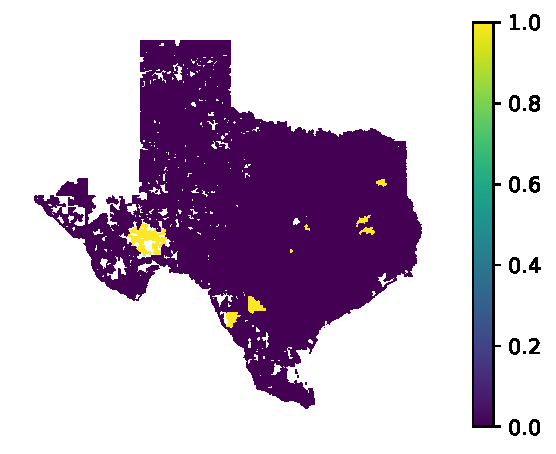
\includegraphics{pset4_template_files/figure-pdf/cell-45-output-1.pdf}

Visually it looks like there are 8 affected zipcodes in Texas.

\begin{Shaded}
\begin{Highlighting}[]
\NormalTok{affected}\OperatorTok{=}\NormalTok{merge\_closures[merge\_closures[}\StringTok{\textquotesingle{}Closures\textquotesingle{}}\NormalTok{]}\OperatorTok{==}\DecValTok{1}\NormalTok{]}
\end{Highlighting}
\end{Shaded}

There are 10 affected zipdoes in Texas. 3.

\begin{Shaded}
\begin{Highlighting}[]
\CommentTok{\#learned that 1 degree is approximately equal to 69 miles}
\CommentTok{\#https://www.google.com/search?q=convert+degrees+to+miles\&rlz=1C1VDKB\_enUS1129US1129\&oq=convert+degrees+to+miles\&gs\_lcrp=EgZjaHJvbWUyCQgAEEUYORiABDIICAEQABgWGB4yCAgCEAAYFhgeMggIAxAAGBYYHjIICAQQABgWGB4yCAgFEAAYFhgeMggIBhAAGBYYHjIICAcQABgWGB4yCAgIEAAYFhgeMggICRAAGBYYHtIBCDUxMjhqMGo3qAIAsAIA\&sourceid=chrome\&ie=UTF{-}8}
\NormalTok{distance}\OperatorTok{=}\DecValTok{10}\OperatorTok{/}\DecValTok{69}
\NormalTok{affected\_buffer}\OperatorTok{=}\NormalTok{affected.copy()}
\NormalTok{affected\_buffer[}\StringTok{\textquotesingle{}geometry\textquotesingle{}}\NormalTok{]}\OperatorTok{=}\NormalTok{ affected\_buffer.geometry.}\BuiltInTok{buffer}\NormalTok{(distance)}
\NormalTok{affected\_buffer.plot().set\_axis\_off()}
\end{Highlighting}
\end{Shaded}

\begin{verbatim}
C:\Users\laine\AppData\Local\Temp\ipykernel_1060\1012217012.py:5: UserWarning: Geometry is in a geographic CRS. Results from 'buffer' are likely incorrect. Use 'GeoSeries.to_crs()' to re-project geometries to a projected CRS before this operation.

  affected_buffer['geometry']= affected_buffer.geometry.buffer(distance)
\end{verbatim}

\includegraphics{pset4_template_files/figure-pdf/cell-47-output-2.pdf}

\begin{Shaded}
\begin{Highlighting}[]
\NormalTok{indirectly\_affected}\OperatorTok{=}\NormalTok{gpd.sjoin(merge\_closures, affected\_buffer, how}\OperatorTok{=}\StringTok{\textquotesingle{}inner\textquotesingle{}}\NormalTok{, predicate}\OperatorTok{=}\StringTok{\textquotesingle{}intersects\textquotesingle{}}\NormalTok{)}
\NormalTok{indirectly\_affected.plot().set\_axis\_off()}
\end{Highlighting}
\end{Shaded}

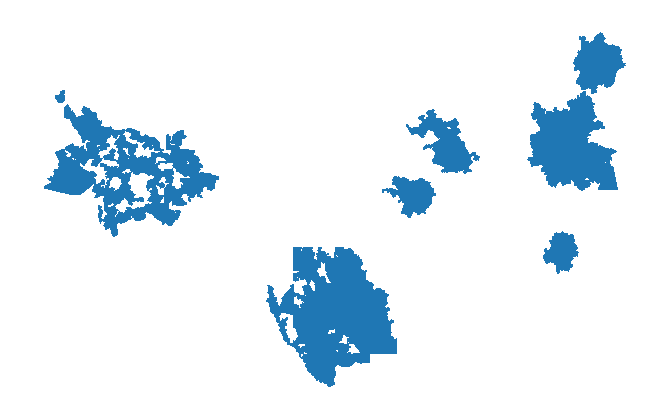
\includegraphics{pset4_template_files/figure-pdf/cell-48-output-1.pdf}

\begin{Shaded}
\begin{Highlighting}[]
\BuiltInTok{len}\NormalTok{(indirectly\_affected)}
\end{Highlighting}
\end{Shaded}

\begin{verbatim}
226
\end{verbatim}

216 zipcodes were indirectly affected. 4.

\begin{Shaded}
\begin{Highlighting}[]
\CommentTok{\#used ChatGPT to debug prompt "merge\_closures[\textquotesingle{}status\textquotesingle{}]=merge\_closures[\textquotesingle{}ZCTA5\textquotesingle{}].map(lambda x: \textquotesingle{}affected\textquotesingle{} if x in affected[\textquotesingle{}ZCTA5\textquotesingle{}] elif x in indirectly\_affected[ZCTA5\_left] \textquotesingle{}indirectly affected\textquotesingle{} else \textquotesingle{}unaffected\textquotesingle{})"}

\NormalTok{merge\_closures[}\StringTok{\textquotesingle{}status\textquotesingle{}}\NormalTok{] }\OperatorTok{=}\NormalTok{ merge\_closures[}\StringTok{\textquotesingle{}ZCTA5\textquotesingle{}}\NormalTok{].}\BuiltInTok{map}\NormalTok{(}
    \KeywordTok{lambda}\NormalTok{ x: }\StringTok{\textquotesingle{}affected\textquotesingle{}} \ControlFlowTok{if}\NormalTok{ x }\KeywordTok{in}\NormalTok{ affected[}\StringTok{\textquotesingle{}ZCTA5\textquotesingle{}}\NormalTok{].values }
    \ControlFlowTok{else}\NormalTok{ (}\StringTok{\textquotesingle{}indirectly affected\textquotesingle{}} \ControlFlowTok{if}\NormalTok{ x }\KeywordTok{in}\NormalTok{ indirectly\_affected[}\StringTok{\textquotesingle{}ZCTA5\_left\textquotesingle{}}\NormalTok{].values }
          \ControlFlowTok{else} \StringTok{\textquotesingle{}unaffected\textquotesingle{}}\NormalTok{)}
\NormalTok{)}
\NormalTok{merge\_closures.head()}
\end{Highlighting}
\end{Shaded}

\begin{longtable}[]{@{}lllllll@{}}
\toprule\noalign{}
& ZCTA5 & geometry & ZIP\_CD & Closures & Texas & status \\
\midrule\noalign{}
\endhead
\bottomrule\noalign{}
\endlastfoot
0 & 78624 & POLYGON ((-98.96423 30.49848, -98.96416 30.498... & 78624 &
0.0 & 0.0 & unaffected \\
1 & 78626 & POLYGON ((-97.60944 30.57185, -97.61688 30.568... & 78626 &
0.0 & 0.0 & unaffected \\
2 & 78628 & POLYGON ((-97.69285 30.57122, -97.69286 30.571... & 78628 &
0.0 & 0.0 & unaffected \\
3 & 78631 & POLYGON ((-99.13053 30.36555, -99.13065 30.365... & 78631 &
0.0 & 0.0 & unaffected \\
4 & 78632 & POLYGON ((-97.40946 29.75929, -97.40947 29.758... & 78632 &
0.0 & 0.0 & unaffected \\
\end{longtable}

\begin{Shaded}
\begin{Highlighting}[]
\NormalTok{merge\_closures.plot(column}\OperatorTok{=}\StringTok{\textquotesingle{}status\textquotesingle{}}\NormalTok{, legend}\OperatorTok{=}\VariableTok{True}\NormalTok{).set\_axis\_off()}
\end{Highlighting}
\end{Shaded}

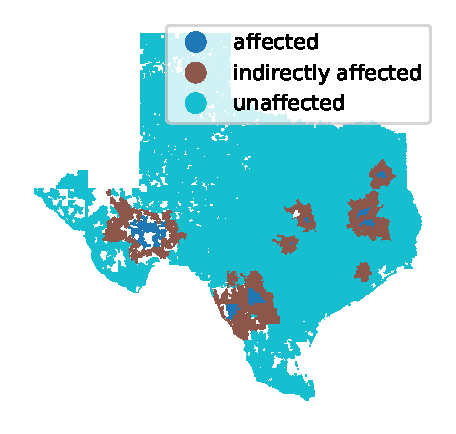
\includegraphics{pset4_template_files/figure-pdf/cell-51-output-1.pdf}

\subsection{Reflecting on the exercise (10
pts)}\label{reflecting-on-the-exercise-10-pts}

Partner 1: While it makes sense to suspect that if the number of active
hospitals didn't decrease, then the hospital was involved in a merger,
this doesn't necessarily have to be the case. A hospital's closure could
be announced some time before the closure actually takes place, and a
new hospital could come in to fill demand. A new hospital could have
come in to the zipcode at the same time that another closed, but with
the first pass method this would be interpretted as the old hospital
being aquired in a merger not a new one taking it's place.

Once we have the list of suspected closures, I think it would be worth
the time to check the facilitiy names of before and after the suspected
closures to see if there are names that are slightly changed. Ex: OSF
St.~Mary to Carle St.~Mary. Since there is a relatively short list of
hospitals suspected of being involved in a merger (13) it wouldn't take
too much time to just Google the hospital individually to see if there
are any reports of a closure or merger.

Partner 2: The existing approach to pinpoint ZIP codes impacted by
hospital shutdowns, which relies on the cessation of hospital operations
between 2016 and 2019, offers a fundamental insight into access
alterations. Nonetheless, it simplifies the effect on healthcare
availability by assuming all closures are the same and not considering
variables like the number of hospitals in each ZIP code, distance to
hospitals in adjacent ZIP codes, or population density.

Way to enhance this is to take into account the number of hospitals
within each ZIP code. A closure in a ZIP code containing many hospitals
might not have as much of an effect as a closure in an area with just
one hospital. Incorporate nearby ZIP codes to evaluate the impact of
closures on access in neighboring areas, since patients may go to other
ZIP codes for healthcare. Integrate population statistics to more
accurately represent the amount of individuals impacted by closures,
particularly in heavily populated regions. These enhancements would
offer a more detailed understanding of the impact of hospital closures
on healthcare accessibility within specific~ZIP~codes.




\end{document}
